\documentclass[a4paper,14pt]{extarticle}
\usepackage[utf8]{inputenc}
\usepackage[russian]{babel}
\usepackage{graphicx}
\usepackage[top=0.8in, bottom=0.8in, left=0.8in, right=0.8in]
{geometry}
\usepackage{pgfplots}
\usepackage{amsmath}
\usepackage{setspace}
\usepackage{titlesec}
\usepackage{float}
\usepackage{chngcntr}
\usepackage{pgfplots}
\usepackage{amsfonts}
\usepackage{pgfplotstable}
\usepackage{multirow}
\usepackage{karnaugh-map}
\usepackage{tikz,xcolor}
\usepackage{indentfirst} % Красная строка
\usepackage{listings}
\usepackage{amssymb}
\usepackage{xcolor}
\usepackage{hyperref}

\definecolor{linkcolor}{HTML}{0000FF} % цвет ссылок
\definecolor{urlcolor}{HTML}{FF00FF} % цвет гиперссылок

\hypersetup{pdfstartview=FitH, linkcolor=linkcolor,urlcolor=urlcolor, colorlinks=true}


\titleformat{\section}[hang]
  {\bfseries}
  {}
  {0em}
  {\hspace{-0.4pt}\large \thesection\hspace{0.6em}}
  
  
\titleformat{\subsection}[hang]
  {\bfseries}
  {}
  {0em}
  {\hspace{-0.4pt}\large \thesubsection\hspace{0.6em}}

%\linespread{1.3} % полуторный интервал
%\renewcommand{\rmdefault}{ftm} % Times New Roman

\newcommand{\nx}{\overline{x}}
\newcommand{\p}{0.31}
\newcommand{\scale}{1.4}

\counterwithin{figure}{section}
\counterwithin{equation}{section}
\counterwithin{table}{section}

\begin{document}
\begin{titlepage}
\centering
Санкт-Петербургский политехнический университет Петра Великого \\
\vspace{0.15cm}
Кафедра компьютерных систем и программных технологий \\
\vspace{6.5cm}

{\centering \textbf{Отчёт по лабораторной работе} \\ 
\vspace{0.15cm}
\textbf{Дисциплина}: Телекоммуникационные технологии \\
\vspace{0.15cm}
\textbf{Тема}: Аналоговая, частотная и фазовая модуляция.} \\


\vspace{6.5cm}

\begin{table}[H]
\begin{tabular}{p{\textwidth}@{}r}
{Выполнил студент гр. 33501/4} \hfill {Мальцев  М.С.} \\
{Преподаватель} \hfill {Богач Н.В.} \\
\end{tabular}
\end{table}
\vfill

{\centering Санкт-Петербург \\ 
\vspace{0.15cm}
\today}
\end{titlepage}

\tableofcontents
\newpage

\section{Цель работы}

Изучение амплитудной частотной и фазовой модуляции/демодуляции сигнала.

\section{Постановка задачи}

\begin{enumerate}
\item Сгенерировать однотональный сигнал низкой частоты.

\item Выполнить амплитудную модуляцию (АМ) сигнала по закону
$$ u(t) = (1 + MU_m cos(\Omega t)) cos(\omega_0 t + \phi_0)$$
для различных значений глубины модуляции M. Используйте встроенную функцию MatLab $ammod$.

Выполнить фазовую модуляцию/демодуляцию сигнала по закону 
$$ u(t) = U_m cos(\Omega t + ks(t)$$
используя встроенную функцию MatLab $pmmod$, $pmdemod$

\item Получить спектр модулированного сигнала.

\item Выполнить модуляцию с подавлением несущей.
$$ u(t) = MU_m cos(\Omega t) cos(\omega_0 t + \phi_0)$$
получить спектр.
\item Выполнить однополосную модуляцию:
$$\displaystyle u(t) = U_m cos(\Omega t) cos(\omega_0 t + \phi_0) + \frac{U_m}{2} \sum^N_{n=1}M_n(cos(\omega_0 + \Omega_n) t + \phi_0 + \Phi_n)$$
положив n=1.

\item Выполнить частотную модуляцию/демодуляцию по закону
$$\displaystyle u(t) = U_m cos(\omega_0 t + k \int_0^t s(t)dt + \phi_0)$$
используя встроенные функции MatLab $fmmod$, $fmdemod$.

\item Выполнить синхронное детектирование и получить исходный
однополосный сигнал.

\item Рассчитать КПД модуляции.
$$\displaystyle \eta_{AM} = \frac{U^2_m M^2/4}{P_U} = \frac{M^2}{M^2 + 2}$$
\end{enumerate}

\section{Теоретический раздел}

\subsection{Модуляция сигнала}



\section{Ход работы}

\subsection{Моделирование синусоидального сигнала}

\subsubsection{Получение непрерывного сигнала}

\begin{figure}[H]
\center{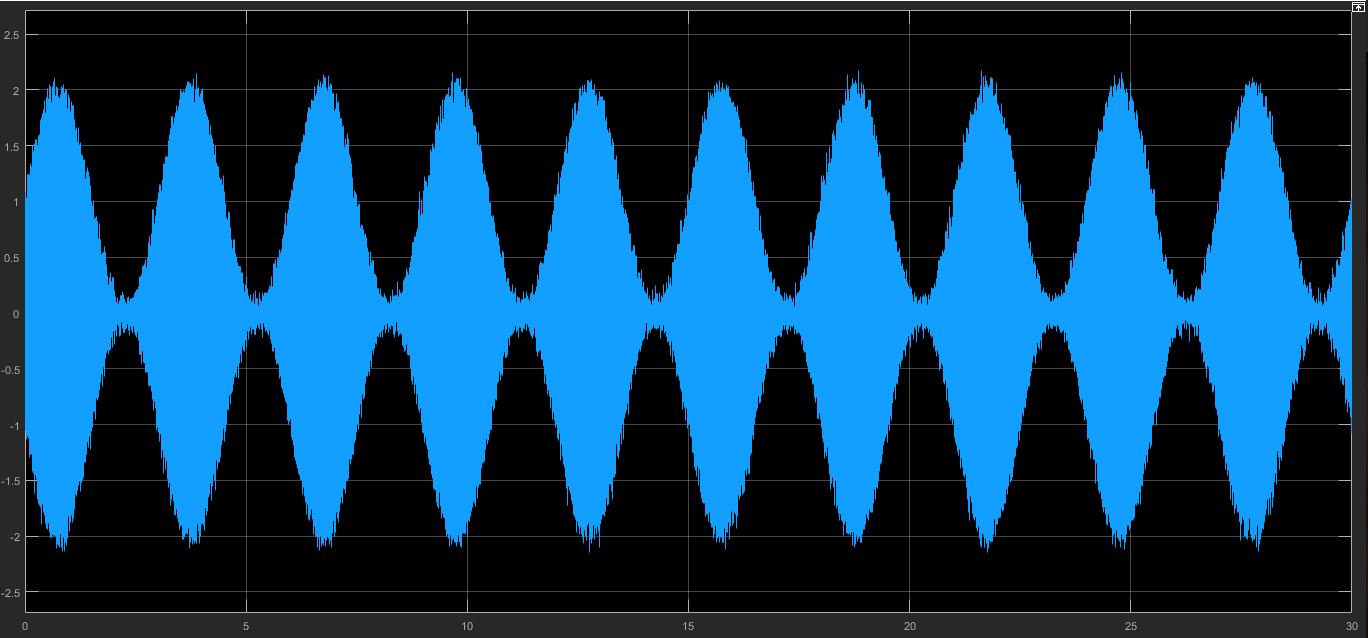
\includegraphics[width=1\linewidth]{img/013.png}}
\caption{Полученный спектр для дискретного прямоугольного 
сигнала. Окно Spectrum Analyzer.}
\label{013}
\end{figure}

\begin{figure}[H]
\begin{minipage}[h]{0.49\linewidth}
\center{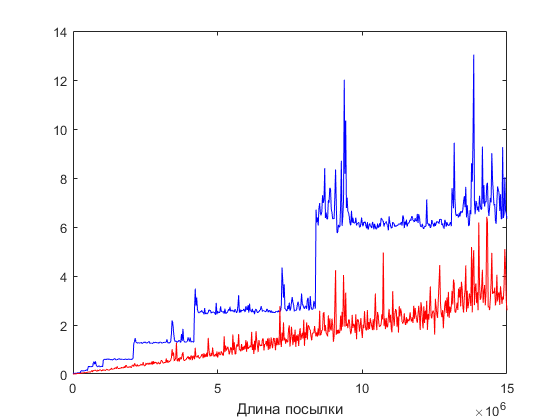
\includegraphics[width=1\linewidth]{img/015_1.png} \\ с шагом 25 000}
\end{minipage}
\hfill
\begin{minipage}[h]{0.49\linewidth}
\center{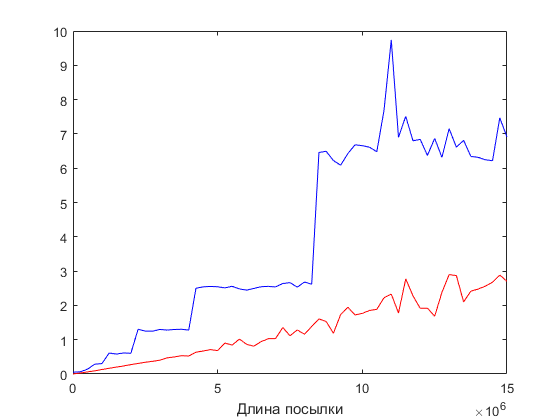
\includegraphics[width=1\linewidth]{img/015_2.png} \\ с шагом 500 000}
\end{minipage}
\caption{Время затрачиваемое на кросс-корреляцию в зависимости от длины посылки}
\label{015}
\end{figure}

\section{Выводы}

\section{Используемые материалы}

\begin{enumerate}

\item \href{https://en.wikipedia.org/wiki/Signal}{Signal (Wikipedia)}

\end{enumerate}

\section{Приложение}

%\lstinputlisting[language=matlab, frame=single, caption=Программа сравнения скорости работы функций, label=lab2_2]{../lab2_2.m}


\end{document}
